\subsection{Vision-Language Models for Document Understanding}

A visual document reader must solve two problems: preserve enough page detail to read the evidence, and expose enough pages to answer the question. These compete for the same image and context budgets. Model size alone does not resolve the trade-off. We organize this section around representation, visual resolution, retrieval granularity and control, using the concrete mechanisms in Table~\ref{tab:visual_document_routes}.

\subsubsection{Representation: Text, Coordinates and Pixels}

Layout-aware encoders preserve explicit word positions; LayoutXLM extends this approach to multilingual documents~\cite{xu2021layoutxlm}. UDOP instead combines text, visual appearance and layout within a generative document processor~\cite{li2022udop}. These interfaces should be distinguished from DocLLM, which generates from text and bounding boxes without an image encoder~\cite{wang2024docllm}. A layout-aware input can retain a column association that plain text loses, but coordinates alone cannot describe a diagram that was never extracted.

Direct-visual readers pass page images to the model. Donut generates structured outputs without a separate OCR engine, while Pix2Struct learns image-to-text parsing through screenshot-based pre-training~\cite{kim2022donut,lee2023pix2struct}. This removes an external transcription stage, rather than the task of reading. Small print, mathematical symbols and relations between distant regions still need to survive image encoding. The practical comparison is therefore between the evidence accessible through each interface, not between an ``OCR'' and ``OCR-free'' label.

The output interface also matters. A document converter must recover content and structure across a page; a question-answering model may only need one value. SmolDocling expresses document elements through DocTags, while general readers such as Qwen2.5-VL and Qwen3-VL support broader visual-language tasks~\cite{kim2025smoldocling,bai2025qwen25vl,bai2025qwen3vl}. A correct answer to one query does not show that the underlying page has been converted completely. Conversely, a complete transcription does not establish that the right evidence was selected for a question.

\begin{table*}[tp]
\centering
\small
\setlength{\tabcolsep}{3pt}
\renewcommand{\arraystretch}{1.15}
\begin{tabularx}{\textwidth}{@{}p{0.18\textwidth}p{0.20\textwidth}XX@{}}
\toprule
Route & Input & Evidence interface & Key constraint \\
\midrule
DocLLM~\cite{wang2024docllm} & Text + boxes & Spatial attention & OCR / layout quality \\
Donut~\cite{kim2022donut} & Page image & Structured generation & Small-text readability \\
mPLUG-DocOwl2~\cite{ye2024docowl2} & Page images & Compressed visual tokens & Detail versus page coverage \\
ColPali~\cite{faysse2024colpali} & Query + page corpus & Ranked multi-vector pages & Index size; retrieval recall \\
VisRAG~\cite{yu2024visrag} & Retrieved images & Selected visual context & Missing evidence pages \\
DocLens / ViDoRAG~\cite{zhu2025doclens,wang2025vidorag} & Adaptive page access & Inspection / retrieval actions & Calls; stopping decisions \\
\bottomrule
\end{tabularx}
\caption{Visual-document interfaces expose different evidence and bottlenecks. Representation, retrieval and adaptive control can be combined within one system.}
\label{tab:visual_document_routes}
\end{table*}

\subsubsection{Visual Budget: Readable Detail versus Page Coverage}

Figure~\ref{fig:visual_budget} illustrates the central resource trade-off. Shrinking a page preserves its overall arrangement but can erase the characters needed to read a footnote. Cropping preserves local detail but requires additional visual tokens and a way to reconnect regions with their source page. A document reader therefore needs both an effective resolution and a policy for allocating that resolution.

\begin{figure*}[tp]
\centering
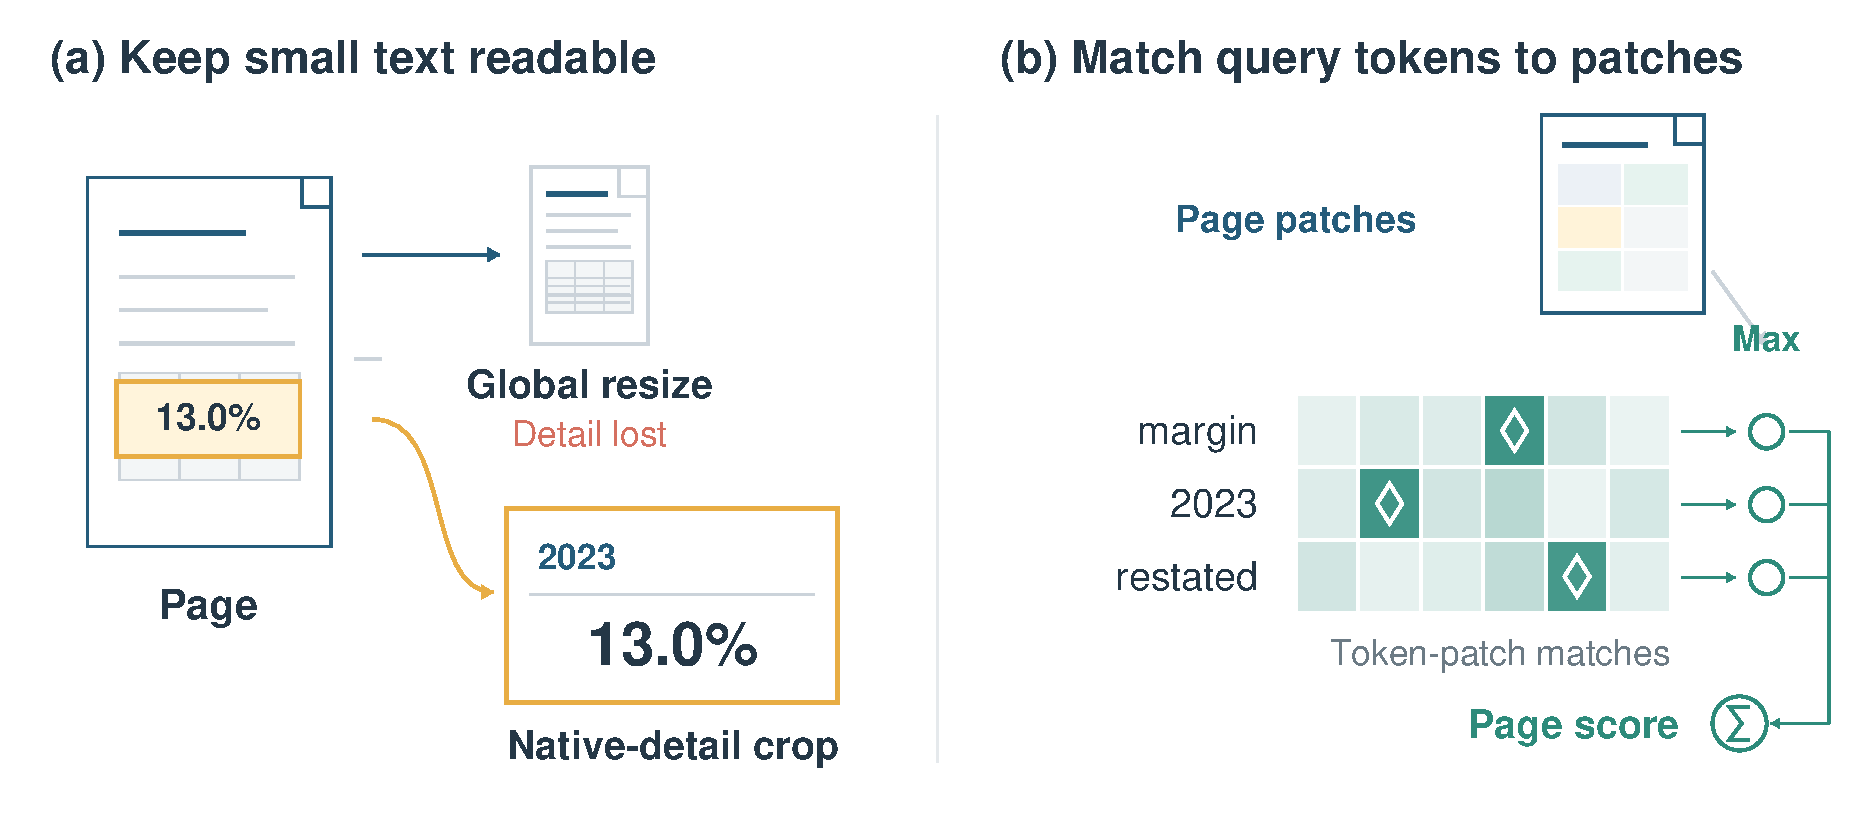
\includegraphics[width=\textwidth]{figs_by_qixingyu/fig15.pdf}
\caption{Two visual-budget decisions: preserve small-text detail through crops, and preserve query-specific matches through patch-level late interaction. The matching matrix is schematic, not a measured retrieval result.}
\label{fig:visual_budget}
\end{figure*}

For a patch encoder, a simple budget model is
\[
N_{\mathrm{visual}} \approx \sum_{p=1}^{P}\sum_{c=1}^{C_p} n_{p,c},
\]
where $P$ is the number of supplied pages, $C_p$ the crops retained from page $p$, and $n_{p,c}$ the tokens for each crop after compression. This accounting separates three choices often hidden behind a maximum-context specification: how many pages are supplied, how finely each is sampled, and how much information the model compresses. It is a resource description, not a performance law.

Monkey and Qwen2-VL study high-resolution or variable-resolution visual processing~\cite{li2024monkey,wang2024qwen2vl}. Structure learning in mPLUG-DocOwl 1.5 and visual slimming in DocKylin address complementary parts of the interface~\cite{hu2024mplugdocowl15,liu2024dockylin}. More pixels can make a character readable; a better representation can make its relation to a header usable. Neither repairs an omitted page. A useful resolution experiment should therefore separate local reading errors from errors caused by missing context.

Coarse-to-fine document conversion offers another allocation strategy: inspect a low-resolution global view, then read selected regions at higher resolution. MinerU2.5 uses this decoupling for document parsing~\cite{liu2025mineru25}. The benefit is selective expenditure of visual computation; the risk is that a region rejected during the coarse pass never receives a detailed reading. Region coverage and reading accuracy should thus be examined together, particularly for small notes and irregular tables.

Multi-page readers add a further compression boundary. mPLUG-DocOwl2 reduces visual-token pressure for multiple images, while Docopilot studies document-level processing as a direct-reading route~\cite{ye2024docowl2,duan2025docopilot}. Their design question differs from single-page OCR: which page details remain distinguishable when many pages share one context? Tests should hold document access constant while varying page count and resolution, rather than supplying one model with a complete report and another with isolated crops.

The original MMLongBench-Doc study illustrates why this distinction matters: 12 of its 14 evaluated LVLMs performed worse than corresponding LLMs given OCR-parsed text~\cite{mmlongbenchdoc2024}. The finding belongs to that study's model versions and budgets. Its broader methodological lesson is to include a strong text-based reader when extracted text contains the required evidence, and to isolate questions that actually depend on visual structure before attributing gains to direct image access.

\subsubsection{Retrieval: Pages, Regions and Cross-Page Evidence}

Visual retrieval indexes page appearance, retaining diagrams and spatial cues that a text-only index may omit. ColPali represents a page with multiple vectors and uses late interaction with query tokens~\cite{faysse2024colpali}. In simplified form, its scoring principle is
\[
s(q,d)=\sum_i \max_j \langle q_i,d_j\rangle,
\]
where each query-token vector $q_i$ matches its most compatible page vector $d_j$. Unlike a single pooled vector, this retains several query-specific matches, with additional index storage and scoring cost.

Document screenshot embeddings offer a unified image-based retrieval input, while VisRAG connects visual retrieval to answer generation~\cite{ma2024unifying,yu2024visrag}. The retrieved object is still an evidence candidate. A relevant page can contain a distracting table, and several individually relevant pages can omit the one footnote needed for a comparison. Retrieval must therefore be assessed both as ranking and as coverage of the complete evidence requirement.

The retrieval unit changes that balance. Page retrieval preserves surrounding context but sends irrelevant content to the reader. RegionRAG selects finer regions; hierarchical indexing in MHier-RAG provides an intermediate organization across document scales~\cite{li2025regionrag,gong2025mhier}. Smaller units improve focus only if headers, units and cross-references survive. For a table cell, the useful evidence unit may be the cell together with its row label, year header and qualifying note, rather than its bounding box alone.

Cross-document systems add evidence composition. M3DocRAG studies visual retrieval over multiple pages and documents, and RAG-Anything organizes heterogeneous content through graph structures~\cite{cho2024m3docrag,guo2025rag}. These mechanisms are useful when a question crosses document boundaries or modalities. Their value should be tested against the simpler alternative of supplying the complete relevant document: retrieval saves context only when the savings outweigh omitted or disconnected evidence.

\subsubsection{Adaptive Access and Stopping}

An adaptive controller chooses what to inspect next after seeing an intermediate result. Figure~\ref{fig:agent_docqa} shows this feedback loop. A search can identify an entity; the next action can open its table, inspect a small note, or execute a calculation. This differs from retrieving a fixed set of pages once, but can use the same underlying OCR, visual encoder and index.

\begin{figure*}[tp]
\centering
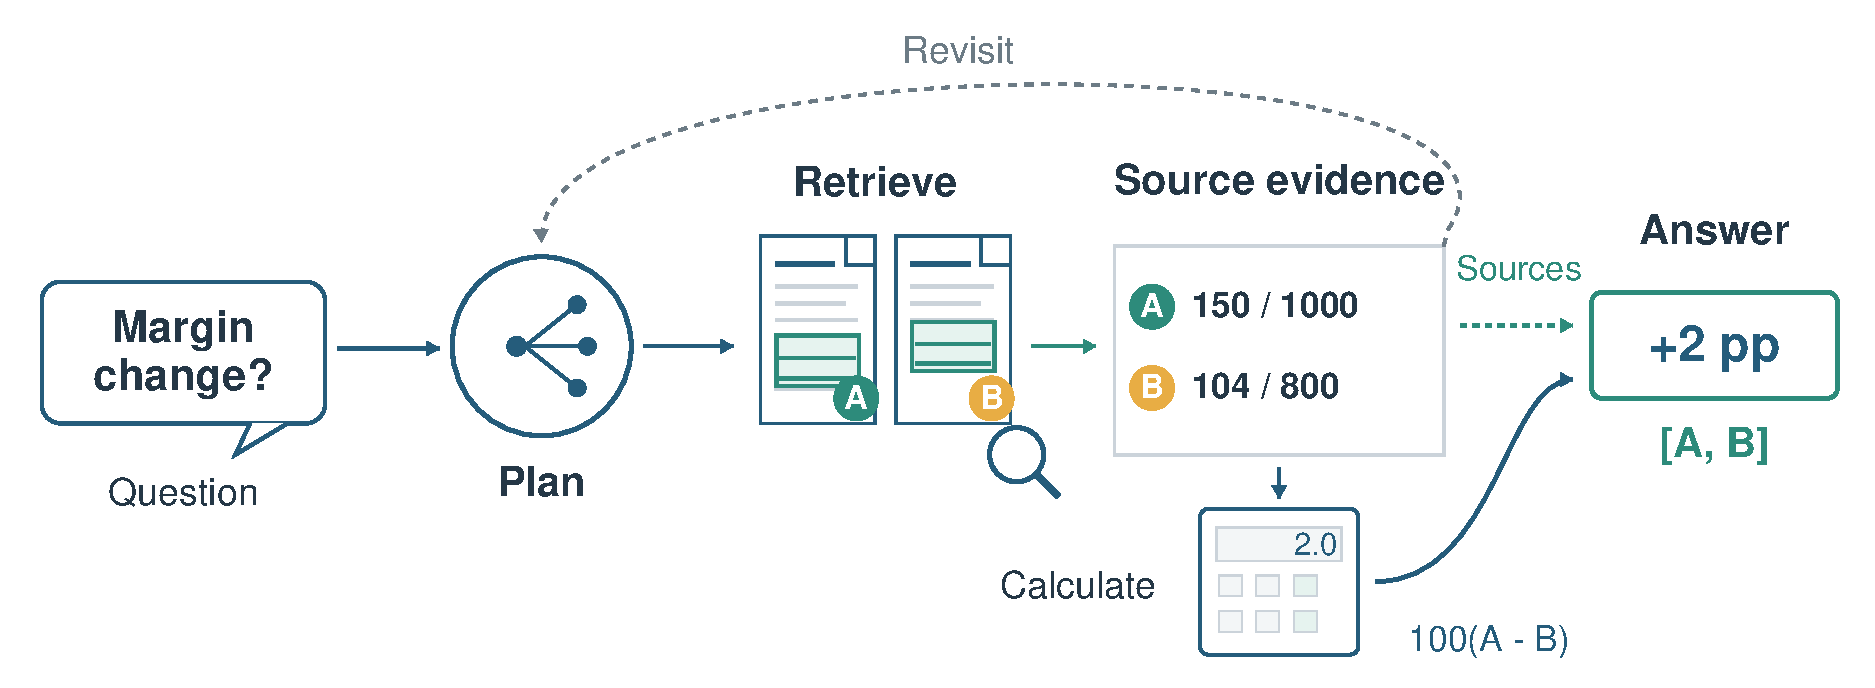
\includegraphics[width=\textwidth]{figs_by_qixingyu/fig08.pdf}
\caption{Adaptive document access links an intermediate evidence need to the next inspection or tool action. The loop ends with supported evidence, an exhausted budget or abstention.}
\label{fig:agent_docqa}
\end{figure*}

DocLens provides tools for inspecting document evidence, while ViDoRAG combines multimodal retrieval with iterative exploration~\cite{zhu2025doclens,wang2025vidorag}. MA-RAG investigates coordinated agents, and CogDoc uses coarse-to-fine reasoning~\cite{nguyen2025ma,xu2025cogdoc}. The shared mechanism is conditional access: later evidence depends on earlier findings. Dividing the same fixed context among several agents is a different intervention and should be compared separately.

A controller also decides how much work a query deserves. AutoThinkRAG explores query-dependent routing of retrieval and reasoning~\cite{autothinkrag}. A direct lookup may need one page; a cross-document comparison may need repeated access. Adaptive effort is most useful when these needs vary across queries. Reporting the average number of calls alone can hide a policy that spends heavily on easy questions and stops early on the difficult ones.

A practical stopping decision asks whether the required evidence has been found and whether the requested operation can be checked. Repeated searches without new support add latency and opportunities for drift. For a small, complete document, a fixed-context reader remains an essential control; for a large collection, fixed retrieval supplies a useful efficiency baseline. Compare these routes under matched page, token and tool budgets, and retain page or region identifiers for the final claims.
